% $Id: CommMem_obj.tex,v 1.2 2003/03/10 03:22:57 cdeluca Exp $

%\section{Object Model}

The core CMK Library consists of six object-oriented classes (types)
as shown in Figure 1 below.  These are:

\begin{itemize}
\item ESMF\_Machine
\item ESMF\_PE
\item ESMF\_DE
\item ESMF\_PEList
\item ESMF\_DELayout
\item ESMF\_Comm
\end{itemize}

These correspond to, and encapsulate the representation and
behavior of, Machine Model, Processor Element (PE), Distributed Element (DE),
Processor Element List (PE List), DELayout, and Communication primitives, as
specified in the ESMF CMK Requirements and ESMF Architecture documents.

\begin{center}
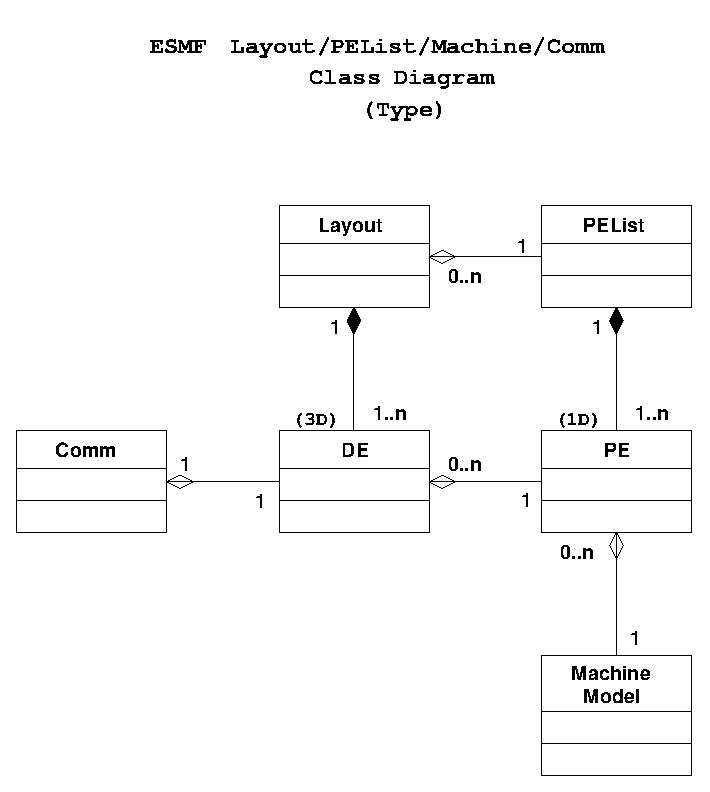
\includegraphics{CommMemClass.EPS}

Figure 1.  ESMF CommMem Class Diagram

\end{center}

\begin{center}
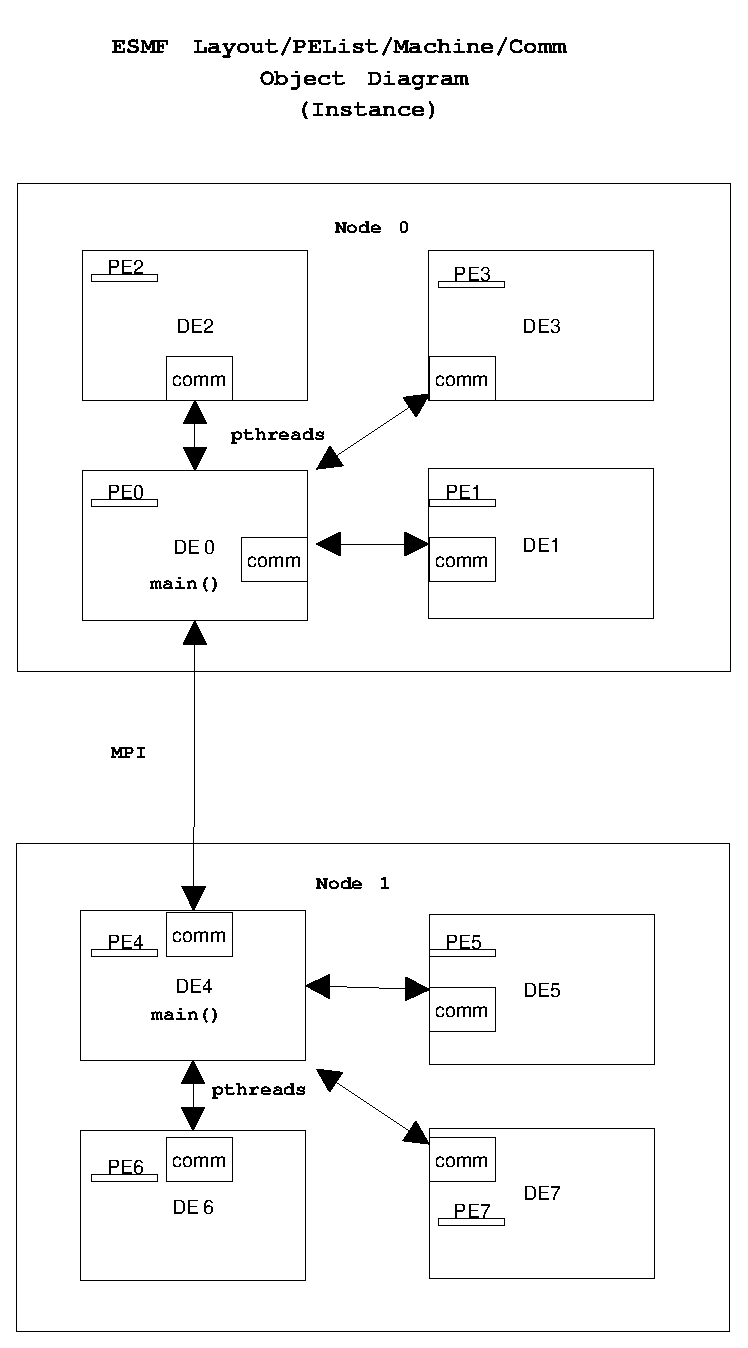
\includegraphics{CommMemObject.EPS}

Figure 2.  ESMF CommMem Example Object Diagram

\end{center}

\begin{center}
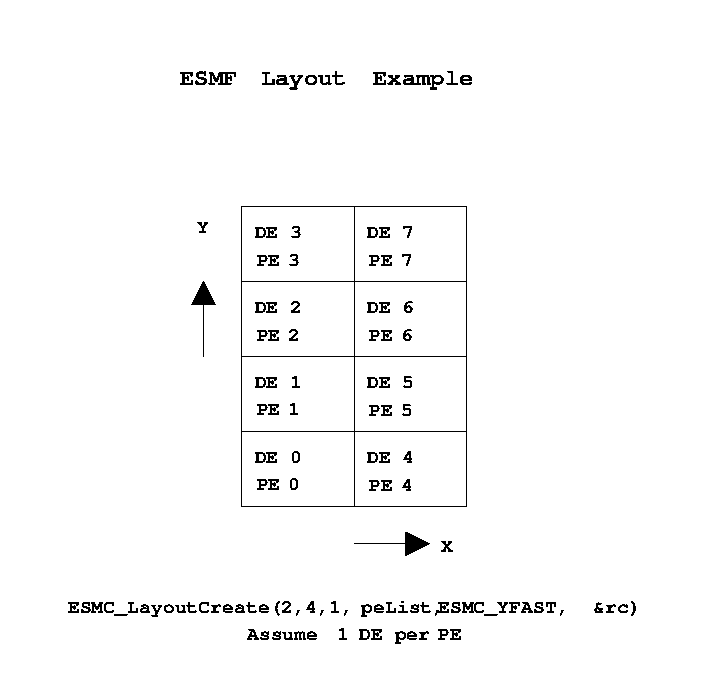
\includegraphics{DELayout.EPS}

Figure 3.  ESMF DELayout Example Object Diagram

\end{center}
